
\documentclass[acmsmall, nonacm]{acmart}


\renewcommand\footnotetextcopyrightpermission[1]{} % removes footnote with conference information in first column
\makeatletter
\let\@authorsaddresses\@empty % removes authors' addresses from first page footer
\makeatother


\usepackage{tikz}
\usetikzlibrary{positioning}
\usepackage{xcolor}
\definecolor{mygreen}{RGB}{0,120,0}
\usepackage{wrapfig}

%% \BibTeX command to typeset BibTeX logo in the docs
\AtBeginDocument{%
  \providecommand\BibTeX{{%
    \normalfont B\kern-0.5em{\scshape i\kern-0.25em b}\kern-0.8em\TeX}}}


\begin{document}


\title{A Divide-and-Conquer Approach to Discovering Minimal Realizable Grammars}


\author{Will Thomas}
\author{Logan Schmalz}
\author{Sarah Johnson}


\maketitle

\section{Introduction}
(Presents the central idea of your project and summarizes the takeaways)

\section{Background}
Our project is based on the work of Semantic-Guided Synthesis (SemGuS) \cite{semgus}. SemGuS aims to be ``a language-agnostic logic-based framework for program synthesis problems over arbitrary semantics''.


\section{Overview}
(Gives step by step working of your project on a single example)

 \begin{wrapfigure}{r}{7.5cm}   
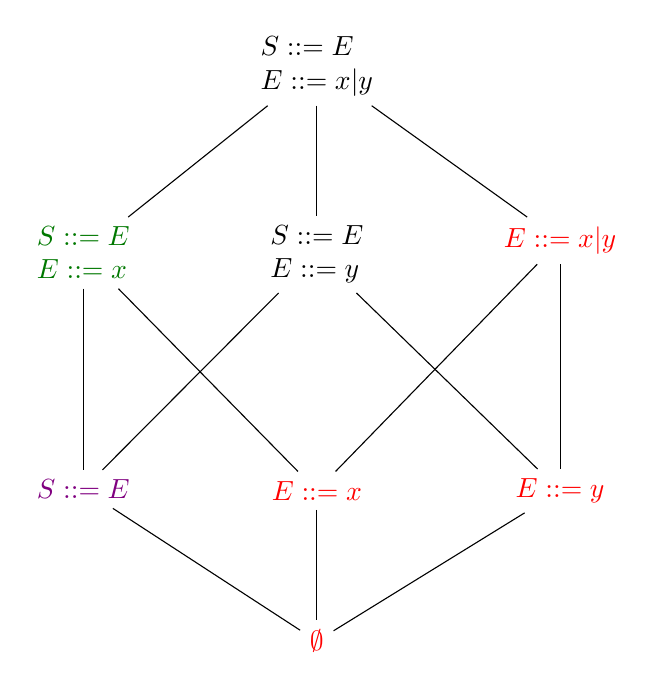
\begin{tikzpicture}[node distance=3cm]
\title{lattice 2}
\node(123)      [align=left]              {$S ::= E$ \\ $E ::= x \text{ }\vert\text{ } y$};
\node(12)       [below left=2cm of 123, align=left] {$\color{mygreen} S ::= E$ \\ $\color{mygreen} E ::= x$};
\node(13)      [below=1.4cm of 123, align=left]  {$S ::= E$ \\ $E ::= y$};
\node(23)      [below right=2cm of 123, align=left]       {$\color{red} E ::= x \text{ }\vert\text{ } y$};
\node(1)      [below of=12]       {$\color{violet} S ::= E$};
\node(2)      [below of=13]       {$\color{red} E ::= x$};
\node(3)      [below=2.6cm of 23]       {$\color{red} E ::= y$};
\node(empty)      [below=1.4cm of 2]       {$\color{red} \emptyset$};

\draw(123)       -- (12);
\draw(123)       -- (13);
\draw(123)       -- (23);
\draw(12)       -- (1);
\draw(12)       -- (2);
\draw(13)      -- (1);
\draw(13)      --  (3);
\draw(23)      --  (2);
\draw(23)      --  (3);
\draw(1)      --  (empty);
\draw(2)      --  (empty);
\draw(3)      --  (empty);
\end{tikzpicture}
\end{wrapfigure}

The problem is to find a minimal realizable grammar to synthesize a function that returns the first projection of an ordered pair. The full grammar consistents of two nonterminal symbols.

\section{Technical Details}
(If your project has formal theory or algorithms you can present it here in the most general form. While the previous section explained the same thing with an example, this section should be about the general technical ideas under the hood)

\section{Implementation}
(The general technical ideas are never enough to get a working implementation :) You probably had to cut corners, optimize certain things to make it practical, etc. which go here)

\section{Evaluation}
 (The results of running your tool, the benchmarks you ran on and your takeaways from it. Things like we learned this parameter is the key bottleneck, our tool struggles on XYZ, or we did well on ABC)

\section{Conclusion}
 (Your concluding take on the project and learnings)

\section{Future Work}
 (Potential future work that you think could be interesting)





\bibliographystyle{ACM-Reference-Format}
\bibliography{projectrefs}


\end{document}

